\chapter{Realizzazione dei prototipi di Power Stack}
Nel corso di questa tesi con la collaborazione dei membri del progetto REGALE, come Cineca\cite{Cineca}, E4\cite{E4} e BSC\cite{BSC} sono stati sviluppati i middleware ed i prototipi di componenti del modello di Power Stack per HPC.
Questi ultimi oltre a fornire una prova delle potenzialità del middleware di DDS, sono utili anche come esempio per una sua effettiva implementazione all'interno dei software mostrati nel capitolo~\ref{chap:4_REGALE} che vogliono essere introdotti nell'infrastruttura.
In merito a questo, nello schema~\ref{fig:schema_global_dummy_implementati} viene mostrato lo stato di avanzamento del Power Stack, illustrando quali di questi sono implementati e operativi, e quali in via di sviluppo.

\begin{figure}[H]
    \centering
    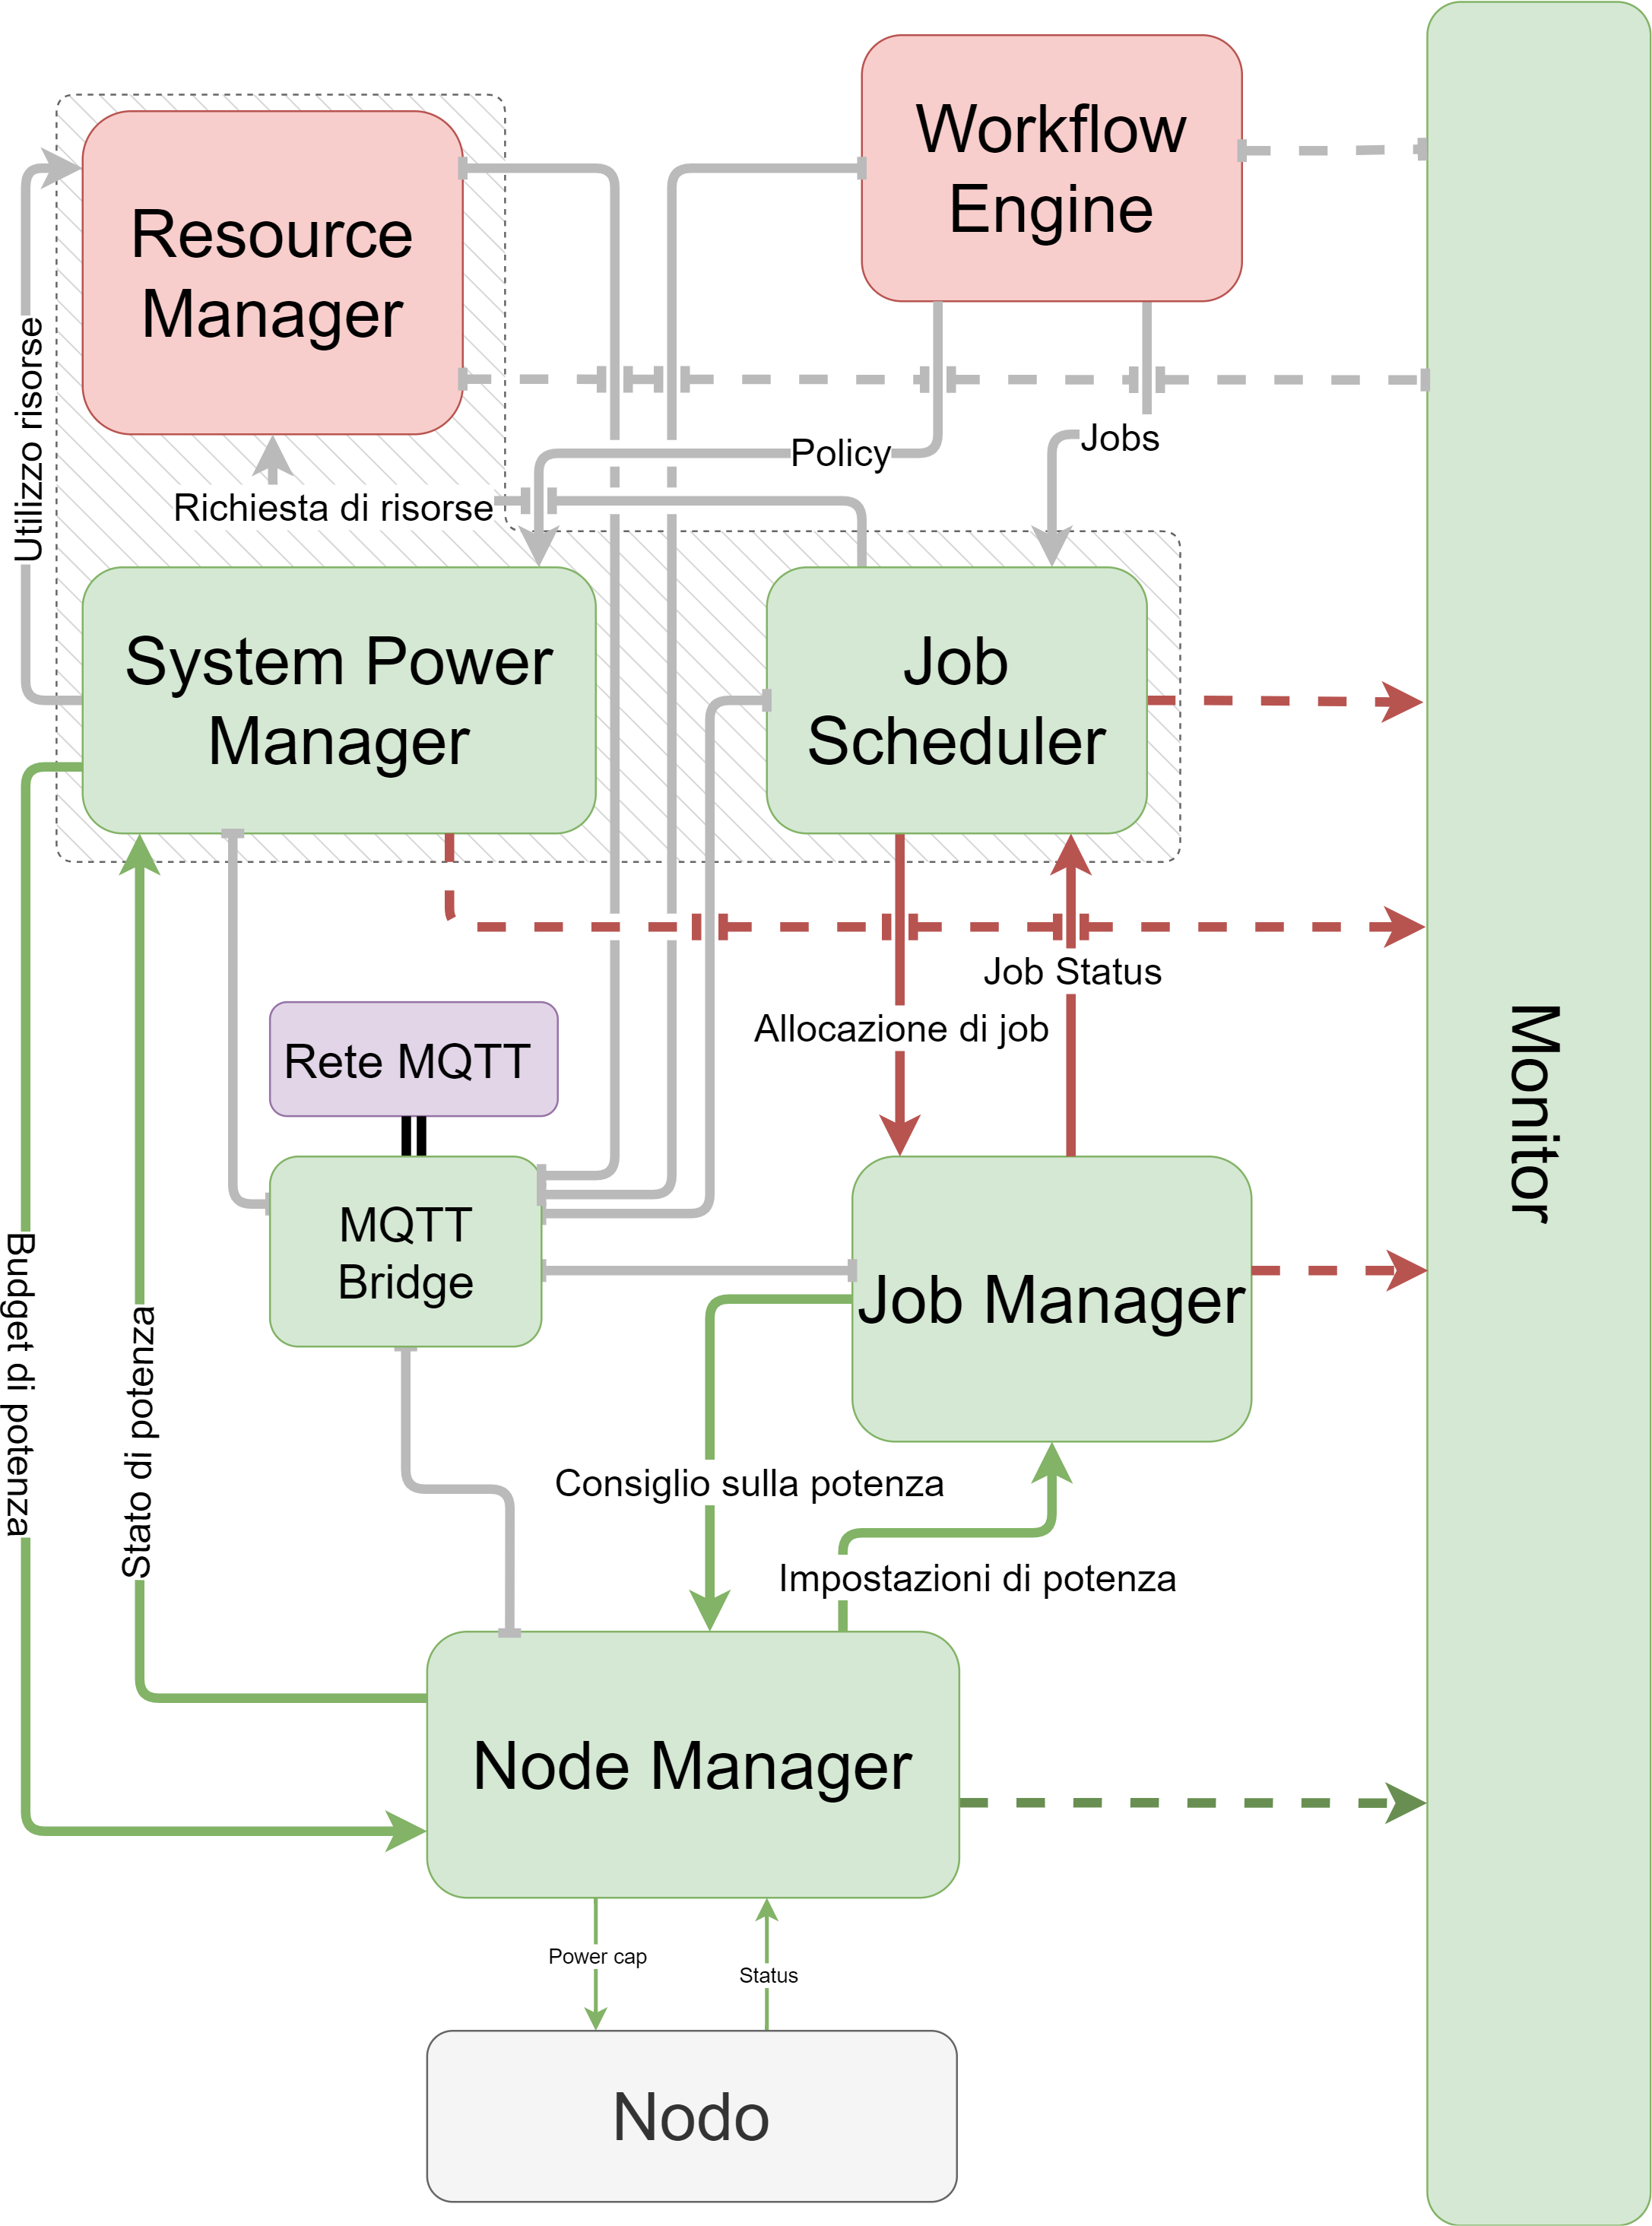
\includegraphics[width=0.5\textwidth]{./img/SchemaPowerStack_perdummy.drawio.png} %TODO: Change
    \caption{Schema componenti sviluppati: in verde completato, in grigio non previsto, in rosso ancora da sviluppare}
    \label{fig:schema_global_dummy_implementati}
\end{figure}
L'infrastruttura DDS creata, chiamata \emph{REGALE Library}\cite{TODO} al momento permette di utilizzare i vari tipi di comunicazione, configurazioni di qos, e anche vari tipi di dati scambiati, tutti passabili tramite file \textbf{XML}.

I prototipi, sono dei programmi in c++ che vanno a simulare uno scambio di informazioni realistico. Al momento per motivi di semplicità utilizzano dati di tipo \emph{uint32\_t} ed il loro comportamento si può riassumere nel seguente modo.

\subsection*{Implementazione Job Scheduler}
Il JS interroga ogni 10 secondi il SPM per le informazioni sui servizi e la potenza totale del cluster riportandolo a schermo. Successivamente  imposta il limite di potenza del cluster con un valore casuale tra 1000 e 1500.

\subsection*{Implementazione Job Manager}
Il JM interroga il NM ogni 10 secondi e richiede il \emph{powercap} impostato e le informazioni sulle frequenze (massima, minima e corrente) riportando a schermo tutti i valori ottenuti.

\subsection*{Implementazione System power manager}
Il SPM nella sua implementazione server aspetta per le richieste in entrata. Al momento quelle previste sono:
\begin{itemize}
    \item GET\_INFO
    \item GET\_POWER
    \item SET\_POWER
\end{itemize}
%  ? Inoltre quando riceve una GET\_POWER il SPM inoltra la richiesta al NM per ottenere la sua potenza prima di rispondere alla richiesta. 

\subsection*{Implementazione Node manager}
Il NM mentre ogni 30 secondi manda i dati al Monitor, aspetta per le richieste in entrata. Le richieste che accetta sono:
\begin{itemize}
    \item GET\_INFO\_NODE
    \item GET\_POWER\_NODE
    \item GET\_POWERCAP\_NODE 
    \item GET\_MINFREQ\_NODE   
    \item GET\_MAXFREQ\_NODE     
    \item GET\_CURFREQ\_NODE   
    \item SET\_POWER\_NODE
\end{itemize}

\subsection*{Implementazione Monitor}
Il Monitor semplicemente aspetta che i componenti gli inviino i dati, e quando li riceve li riporta a schermo.

\subsection*{MQTT Bridge}
Questo componente, a differenza di tutti gli altri, non ha alcun ruolo nel Power Management ma serve solo a supporto di alcuni software che fanno ampio uso di comunicazioni \textbf{MQTT}\cite{mqtt}. Infatti il suo scopo è quello di intercettare e convertire tutte le comunicazioni provenienti da MQTT e DDS per infine inoltrare quelle desiderate nel protocollo opposto (DDS in MQTT e viceversa).% Come dice il nome fa da \emph{ponte} tra le due infrastrutture, semplificando l'introduzione di alcuni software come Countdown\cite{cesarini2019countdown}.

\section{Struttura}
I componenti mostrati, al momento fanno uso delle strutture di domini, partizioni e topic mostrati in tabella~\ref{fig:dummy_topic}.

\begin{figure}[H]
    \centering
    \includegraphics[width=0.75\textwidth]{./img/server\_skeleton.png}
    \includegraphics[width=0.75\textwidth]{./img/dummies\_skeleton.png}
    \caption{ Strutture di comunicazioni dei componenti implementati nel power stack.}
    \label{fig:dummy_topic}
\end{figure}
% In viola tutti i publisher, ed in giallo i subscriber. Successivamente nel rispettivo ordine vengono mostrati, domini, partizioni e topic utilizzati.
